\documentclass[14pt]{extarticle}
\usepackage[T2A,T1]{fontenc}
\usepackage[english,russian]{babel}
\usepackage{graphicx}
\usepackage{tikz-qtree}
\usepackage{listings}
\usepackage{mathtools}
\usepackage{circ}
\usepackage{yhmath}
\usepackage[margin=2cm]{geometry}
\DeclarePairedDelimiter{\ceil}{\lceil}{\rceil}

    \title{\textbf{Решение ЕГЭ Информатика}}
    \author{Юрченко Александр 11 "А"}
    \date{}
    
    \setlength{\headheight}{0.6pt} 
	%\setlength{\headsep}{-2cm}
	%\setlength{\topmargin}{-2pt}
	%\setlength{\marginparsep}{11pt}

\begin{document}
	
\maketitle
\newpage
\thispagestyle{empty}

\section{№1}
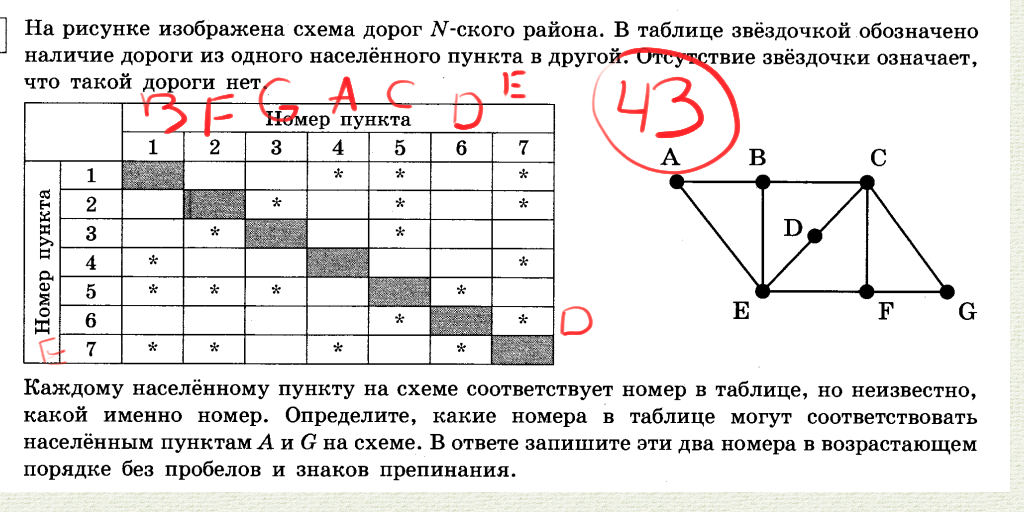
\includegraphics[scale=0.5]{1.png}

Ответ: 43

\section{№2}
Код:
\begin{lstlisting}[language=Python]
def f(x,y,z,w):
    return not(x<=y) or (x==z) or w

print("x y z w")
for x in range(2):
    for y in range(2):
        for z in range(2):
            for w in range(2):
                tmp = f(x,y,z,w)
                if tmp==0:
                    print(x,y,z,w,tmp)
"""
x w z y f()
1 0 0 1  0
0 0 1 1  0
0 0 1 0  0
"""

\end{lstlisting}

Ответ: xwzy
\section{№3}

Ответ: 18920
\section{№4}
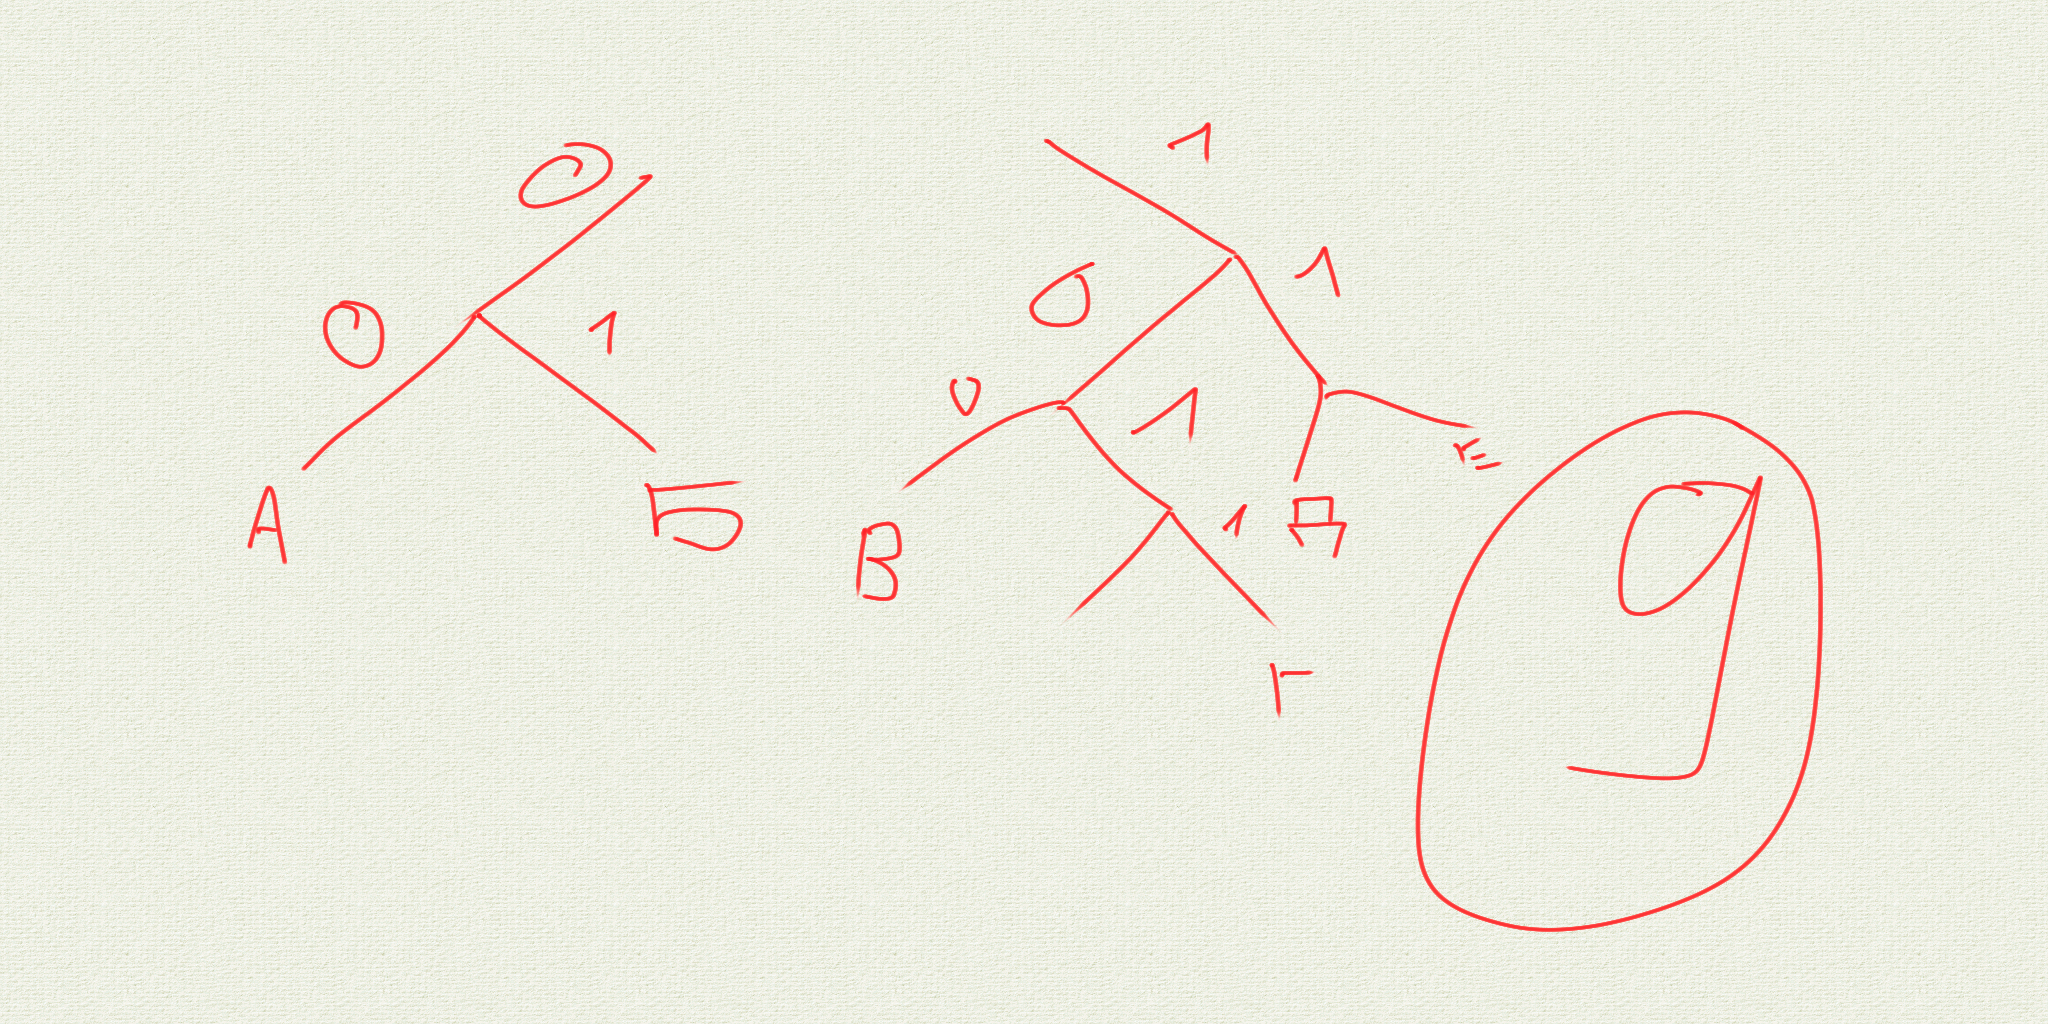
\includegraphics[scale=0.3]{4.png}
Ответ: 9

\section{№5}
\begin{lstlisting}[language=Python]
def f(n):
    res=""
    stm="0123"
    while n!=0:
        res=stm[n%4]+res
        n//=4
    return res

for n in range(1,10000):
    r=f(n)
    if n%4==0:
        r+=r[-2:]
    else:
        r+=f(n%4*2)
    if int(r,4)<261 :
        print(int(r,4))
\end{lstlisting}
Ответ: 246

\section{№6}
Ответ: 

\section{№7}

\begin{align*}
	\intertext{Пусть} pixels &= 480*270 \text{, } depth = 4*2^3 \text{ и } V = 14400 \text{ бит/с} \intertext{тогда}
	t &= \frac{pixels * depth}{V}=288c
\end{align*}
Ответ: 288

\section{№8}

\newcommand{\isPrime}[1]{isPrime\left(#1\right)}

\begin{lstlisting}[language=Python]
    from itertools import product
    words=0
    count=1
    for i in product("favorit", repeat=6):
        if(count%2==0):
            if(i[0]!='o'):
                if(i.count("r")==2):
                    words+=1
        count+=1
    print(words)
\end{lstlisting}
Ответ: 8640


\section{№9}

Ответ:

\section{№10}
Ответ: 255-197 = 58

\section{№11}
Пусть $N=60+10 \text{, } length=108 \text{ и } n = 25600$
\begin{align*}
\intertext{Найдем необходимое место для одного id (в байт)}
& size_{id} = \ceil{\frac{\ceil{\log_{2}{N}}*length}{2^3}} \\
& answer = \frac{\displaystyle n*size_{id}}{2^{10}}
\end{align*}
Ответ: 496



\section{№12}
\begin{lstlisting}[language=Python]
    for n in range(3,10000):
    s = "1" + "2"*n
    while "12" in s or "3322" in s or "2222" in s:
        if "12" in s:
            s=s.replace("12", "33", 1)
        if "22222" in s:
            s=s.replace("2222", "1", 1)
        if "3322" in s:
            s=s.replace("3322", "21", 1)
        arr = list(map(int, s))
        if sum(arr)==218:
            print(n)    
\end{lstlisting}
Ответ: 177

\section{№13}
Ответ: 
\section{№14}
\begin{lstlisting}[language=Python]
for x in "0123456789abcdefghijklm":
    if (int(f"1{x}1{x}1{x}1{x}1{x}",23)+int(f"20{x}24",23)+int(f"1{x}235",23)) % 22==0:
        print(x)
\end{lstlisting}
Ответ: 6
\section{№15}
Ответ:

\section{№16}
\begin{lstlisting}[language=Python]
f=[0]*30000

f[1]=5
for i in range(2,2030):
    f[i]=2*i+1+f[i-1]
print(f[2024]-f[2022])
\end{lstlisting}
Ответ: 8096

\section{№17}

\begin{lstlisting}[language=Python]
file = open("../files/17.txt")
data = list(map(int, file.readlines()))
count = 0
mn_25 = 10**7
mxsum=0
for i in data:
    if i%100==25:
        mn_25=i

for i in range(len(data)-2):
    a,b,c=data[i], data[i+1], data[i+2]
    if list(map(len, map(str, map(abs, [a,b,c])))).count(2)==1:
        if a+b+c<mn_25:
            count+=1
            if mxsum<a+b+c:
                mxsum=a+b+c
print(mxsum, count)
\end{lstlisting}

Ответ: 81093 1691
\section{№18}
Ответ: 588 210
\section{№19-21}
Ответ: 
67;
63 66;
65;



\end{document}